\subsection{Maze Structure}
\begin{figure}[h]
\center
\includegraphics[scale=0.25]{top_view_lowres.png}    
\caption{Top View of the maze}
\end{figure}
\justify The figure above shows the detailed description of the maze used in the project. The dimensions of the maze walls are described in the figure as well. All the walls in the maze have a uniform height of 6 inches. The width of the path that the robot drives in is 14.2 inches wide. The appropriate distance between the two walls for the robot to drive through was selected by a trial and error process where the robot was made to run in paths of various widths. Suitable width was required for the robot to make the U-turn properly without making contact with the walls. Similarly, the sensing distance for the right and left sensors was kept in mind while determining the width.\\
For the purpose of implementing “Left Wall Following” algorithm, a simply connected maze was designed. This means that all the walls of the maze are connected together. 
The start point of the maze is selected as shown in the figure. Similarly, the target is placed along one of the maze boundaries. The dimensions of the maze is summarized below:
\begin{itemize}
\item Wall height – 6 inches
\item Width between two walls – 14.2 inches
\item Total length along the longest side – 124.8 inches 
\item Total width – 68.4 inches
\end{itemize}
\justify The maze is designed in such a way that when the first robot traverses through it, it goes through multiple U-turns and commits several mistakes before finally reaching the target. This way, when the shortest path to the target is decoded, the second robot does not go through any U-turn and follows a simple path to the target.\\
The maze structure was designed using AutoCAD and its 3-dimensional model is shown below:
\begin{figure}[h]
\center
\includegraphics[scale=0.6]{maze2.jpg}   
\caption{Angular View of the maze}
\end{figure}
\subsection{Configuration of Robots}
The robots used as the agents of the swarm are two differentially driven robotic vehicles as shown in the figure. The rear wheel are driven by the PWM signal generated at the processor, which in our case is the Arduino.\\
Both the agents have two rear wheels which are rotated using a DC motor each mounted on the axle of the wheel. The degree of freedom for each of the rear wheel is two i.e. it can be rotated or moved in two direction viz. forward and backward. The rear wheels are composed of plastic tire surrounding the circular frame as shown in the figure.
\begin{figure}[h]
\center
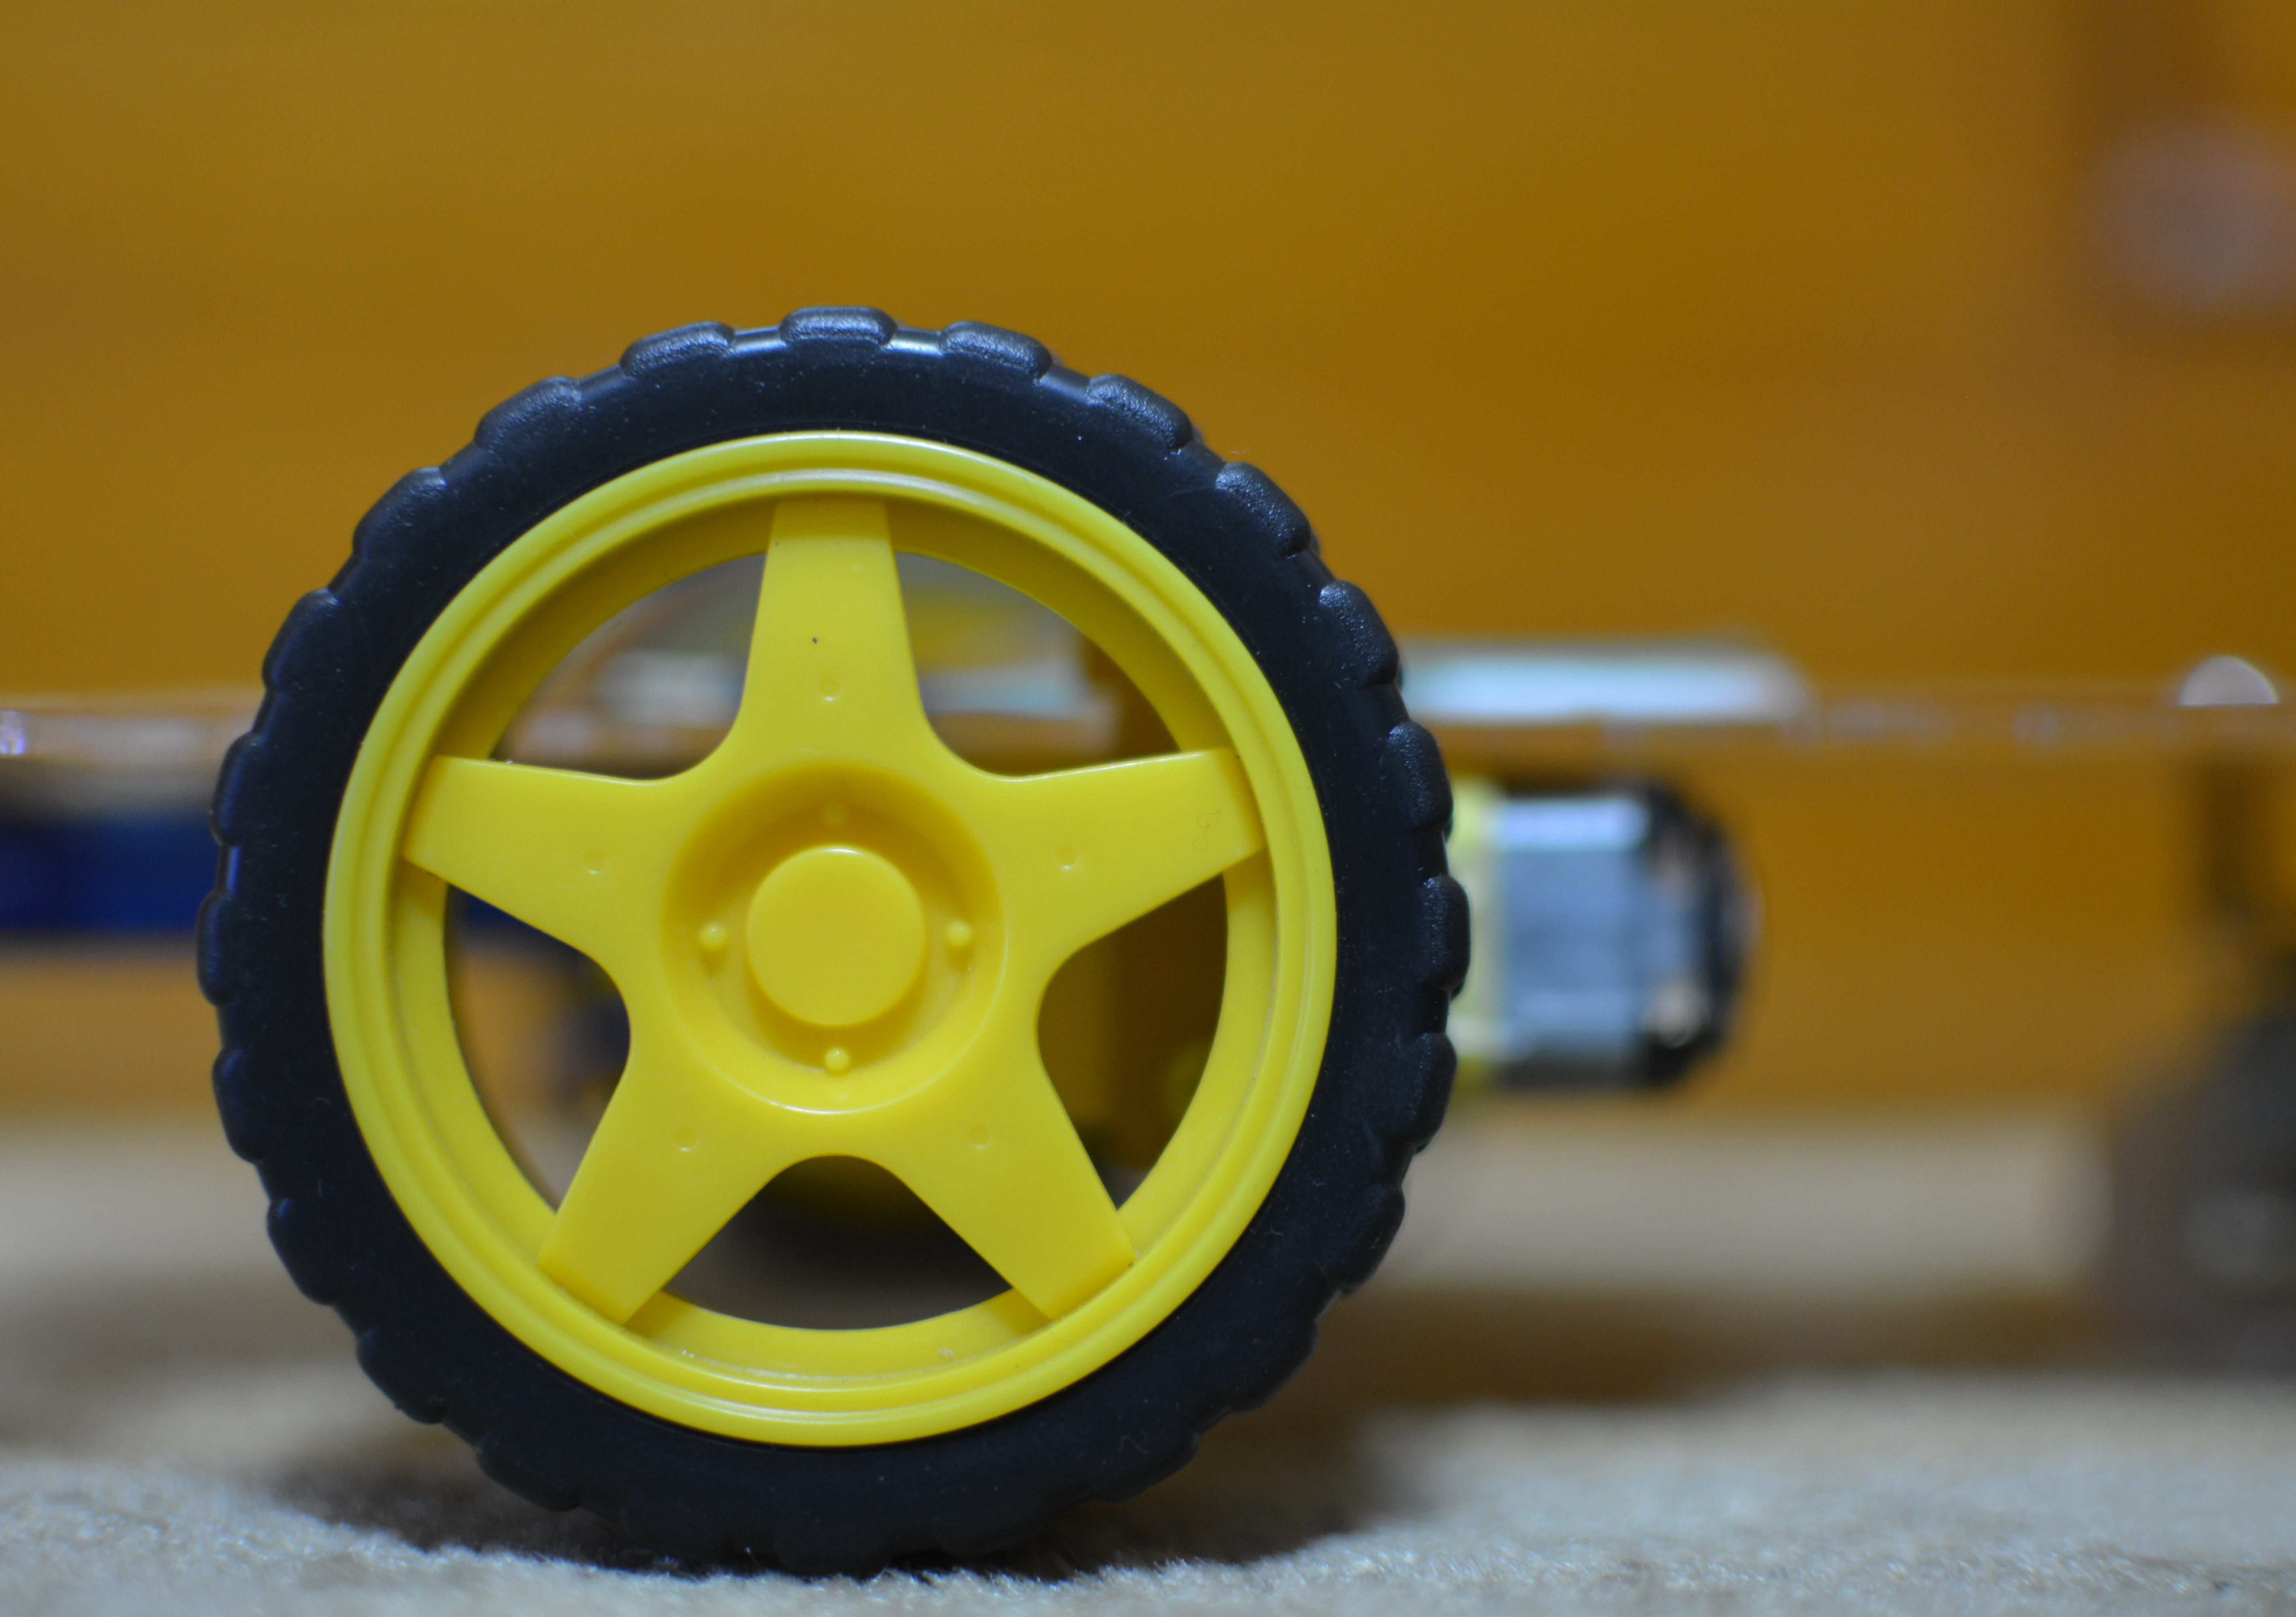
\includegraphics[scale=0.25]{DSC_0023.JPG}    
\caption{The wheel of the robot}
\end{figure}
\justify At the front end of the robots is a caster ball wheel. In this type of wheel, a spherical metal ball is held within a vertical holder. The caster ball wheel helps balancing the robot. The use of the caster ball wheel can be justified as our project is not concerned with the motion in the rough terrain.
\newpage
\begin{figure}[h]
\center
\includegraphics[scale=0.5]{caster.JPG}    
\caption{Caster wheel used in the robot}
\end{figure}
\justify The physical dimensions of the different parts of the robot are tabulated below:
\begin{table}[h]
\begin{center}
\begin{tabular}{|c|c|}
\hline
Length of robot	&8.27”\\
\hline 
Width of robot	&3.93” at the shorter side / 5.9” at the longer side\\
\hline 
Diameter of rear wheels	& 2.52”\\
\hline 
Diameter of front caster wheel&	11mm\\
\hline
\end{tabular}
\end{center}
\caption{The physical dimension of the robot}
\end{table}
\justify The electrical properties of the robot is described in the table below:
\newpage
\begin{table}
\begin{center}
\begin{tabular}{|c|c|}
\hline
Total source voltage &7.4V\\
\hline
Voltage to Arduino &5V\\
\hline 
Voltage to IR sensor& 5V\\
\hline 
Voltage to Smoke sensor& 5V\\
\hline 
Voltage to Bluetooth &3.3V\\
\hline 
Current to each IR sensor& 43mA\\
\hline 
Total current to all IR sensors& 43*3mA = 129mA\\
\hline 
Current through Smoke sensor &800mA\\
\hline
\end{tabular}
\end{center}
\caption{The electrical properties of the robot}
\end{table}
\subsubsection{First Robot}
Aside from the descriptions for the robot given above, the first robot consists of several sensor modules. It has 3 IR sensors attached at the front, left and right sides of the body. The smoke sensor is also attached at the front end besides the IR sensor. Similarly, the bluetooth module HC-05 is attached at the rear end of the robot . With the motor controller attached at the centre of the body and the arduino behind it, the battery had to be attached at the back side of the robot.\\
The entire body is made up of acrylic. Small holes are drilled at various locations in the body which allows the sensors and modules to be attached firmly. 
\newpage
\begin{figure}[h]
\center
\includegraphics[scale=0.25]{bot1new.jpg} 
\caption{Schematic Representation of the first Robot}
 \end{figure}
\subsubsection{Second Robot}
The second robot is not much different from the first one. In the process of describing swarm intelligence, the second robot is intentionally made simpler than the first robot. So, tit does not contain the smoke sensor. Three IR sensors are attached just as in the first robot. Similarly, the arduino, bluetooth module and the motor controller are also attached in a similar way.The schematic is shown below:
\begin{figure}[h]
\center
\includegraphics[scale=0.25]{bot2new.jpg} 
\caption{Schematic Representation of the second Robot}
 \end{figure}
\subsection{Interfacing Arduino UNO with L298N Dual H-Bridge motor controller}
Common Ground technique was applied by connecting the GND terminal of the UNO's to the ground socket of the motor controller. The supply to the UNO was provided via the 5v output socket of the motor controller and the motor controller was powered with Lithum Polymer battery.\\
For the interfacing of Arduino UNO with the L298N, the following pin configurations were done:
 
\begin{table}[h]
\center
\begin{tabular}{ |p{3cm}|p{3cm}|p{3cm}| }
\hline
\multicolumn{3}{|c|}{PIN CONFIGURATION} \\
\hline
ARDUINO PIN& L298N PIN &Remarks\\
\hline
5(PWM) & IN4&Enable Motor B\\
\hline
6 & IN3&Enable Motor B\\
\hline
7 &IN2&Enable Motor A \\
\hline
8 &IN1 &Enable Motor A\\
\hline
9&ENB&Enables PWM signal for Motor B.\\
\hline
10(PWM)& ENA& Enables PWM signal for Motor A \\
\hline
\end{tabular}
\caption{Pin Configurations of the interfacing of ArduinoUNO with L298N}
\end{table}
